\clearpage
\section{Technische Grundlagen Thread}\label{sec:TechnischeGrundlagenThread}
In der Abbildung \ref{fig:ÜbersichtThreadProtokoll} ist zu sehen, wie das Thread Protokoll aufgebaut ist. In den folgenden Unterkapiteln wird auf die verschiedenen Layer des Stacks eingegangen.
\begin{figure}[H]
	\centering
	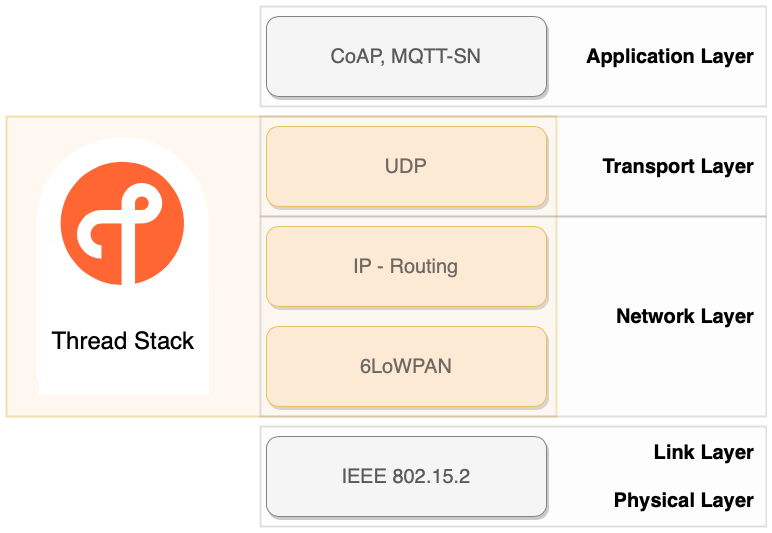
\includegraphics[width=0.6\textwidth]{Overview Thread.png}
	\caption{Übersicht Thread Protokoll}\label{fig:ÜbersichtThreadProtokoll}
\end{figure}

\subsection{Application Layer}\label{subsec:CoAP}
Da das Thread Protokoll auf einer UDP Kommunikation basiert, ist die Wahl des Applikation Layers, dem Entwickler freigestellt. Grundsätzlich ist jedes Protokoll einsetzbar, dass auf einer UDP-Kommunikation basiert. Da Thread das Netzwerkmanagement über das Constrained Application Protocol (CoAP) abfertigt, wird CoAP in diesem Kapitel etwas näher erläutert.

\subsubsection{CoAP}\label{subsubsec:CoAP}
Das Constrained Application Protocol (CoAP) ist ein spezialisiertes Web-Übertragungsprotokoll das dafür entwickelt wurde, um eingeschränkten Geräten die Teilnahme am IoT zu ermöglichen. CoAP ist durch seinen niedrigen Stromverbrauch und geringen Netzwerk-Overhead dafür ausgelegt bei einem Netzwerk mit kleiner Bandbreite und hoher Auslastung zu funktionieren.  UDP wird als grundlegendes Netzwerkprotokoll verwendet, das bedeutet das CoAP ein Client-Server-IoT Protokoll ist, welches die gleichen Methoden wie HTTP verwendet. Das Protokoll wird für Machine-to-Machine (M2M)-Anwendungen wie intelligente Energie- und Gebäudeautomatisierung verwendet. Dank diesen Eigenschaften ist es möglich CoAP bei Stromsparenden Modulen einzusetzen, während TCP-basierte Protokolle nicht in der Lage sind Informationen auszutauschen. Das Protokoll wurde von der Internet Engineering Task Force (IETF) entworfen, CoAP ist in IETF RFC 75852 spezifiziert. In der Tabelle \ref{table:FeaturesCoAP} sind einige Features aufgelistet. \cite{shelby_constrained_2014}

\begin{table}[H]
	\centering
	\begin{adjustbox}{width=1\textwidth}
		\begin{tabular}{@{}|l|l|l|@{}}
			\toprule
			\multicolumn{3}{|c|}{\textbf{Features}}                                                             \\ \midrule
			Web-Protokoll M2M                & Geringer Overhead               & Proxy- und Caching Fähigkeiten \\ \midrule
			Asynchroner Nachrichtenaustausch & URI Uniform Resource Identifier & User Datagram  Protocol  (UDP) \\ \bottomrule
		\end{tabular}
	\end{adjustbox}
	\caption{Features CoAP}
	\label{table:FeaturesCoAP}
\end{table}
\newpage


\subsection{Thread Protokoll Stack}\label{subsec:ThreadProtokollStack}
Der Thread Stack besteht im Grunde aus den beiden Transport und Network Layer (Abbildung \ref{fig:ÜbersichtThreadProtokoll}). Dank dieser Schicht ist es möglich eine geroutete IPv6-Verbindung mit verschiedenen IoT fähigen Geräten aufzubauen. Nachfolgend wird erläutert, wie der Stack aufgebaut ist.

\subsubsection{UDP}\label{subsubsec:UDP}
Das Thread Protokoll schreibt vor, dass ein User Datagram Protocol (UDP) nach dem Standard \cite{postel_user_1980} implementiert werden muss. UDP ist ein minimales und verbindungsloses Netzwerkprotokoll, das ein Versand von Datagrammen innerhalb IP-basierten Netzwerken ermöglicht. Das Protokoll verwendet Ports um die Nachrichten an die richtigen Empfänger zu versenden. Zusätzlich besteht die Möglichkeit eine Prüfsumme mit der Nachricht zu versenden, um Fehlerhafte Nachrichten zu identifizieren. \cite[Seite 6-2]{thread_group_inc_thread_2017}

\subsubsection{IP Routing}\label{subsubsec:IPRouting}
Das Thread Routing-Protokoll ist ein einfaches Distanz-Vektor-Routing-Protokoll. Das Ziel ist es die Routing-Information, die mit einer Nachricht versendet werden kann, zu erhöhen. Aus diesem Grund ist die Anzahl Router im Netzwerk limitiert. Alle Router versenden periodisch ihre Link-Kosten und die Verbindungsqualitäten zu direkt erreichbaren Routern im ganzen Netz. Die endgültigen Routing-Kosten zu einem Ziel, sind demnach die Kosten von allen Routern zum Ziel plus die Kosten zum direkten Nachbarn. Mit dem Trickle-Algorithmus \cite{levis_trickle_2011} wird die Rate festgelegt mit der ein Router seine Informationen ins Netz sendet. \cite[Seite 5-23]{thread_group_inc_thread_2017}

\subsubsection{6LoWPAN}\label{subsubsec:6LoWPAN}
6LoWPAN (IPv6 over Low-Power Wireless Personal Area Networks) ist ein drahtloses Low-Power-Mesh-Netzwerk, bei dem alle Knoten über IPv6-Adressen kommunizieren. Ein Thread Gerät muss das Protokoll implementiert haben. 6LoWPAN dient als Anpassungsschicht zwischen dem MAC Layer und dem Netzwerk Layer. Das Protokoll fragmentiert und setzt die IPv6-Pakete wieder zusammen, damit die grösse der payload vom IEEE 802.15.4 Protokoll übereinstimmt. 6LoWPAN adaptiert somit die IPv6-Pakete auf die IEEE 802.15.4 Pakete, die von der Radioschnittstelle gesendet werden. \cite{thubert_compression_2011} In der Tabelle \ref{table:Features6LoWPAN} sind einige Features aufgelistet. \cite[Seite 3-10]{thread_group_inc_thread_2017}
\begin{table}[H]
	\centering
	\begin{adjustbox}{width=1\textwidth}
		\begin{tabular}{@{}|l|l|l|@{}}
			\toprule
			\multicolumn{3}{|c|}{\textbf{Features}}                                                      \\ \midrule
			Offene IP Standards         & Unterstützt Schlafende Endgeräte & Skalierbares Mesh-Routing   \\ \midrule
			End-Zu-End IP Kommunikation & Selbst Heilendes Netzwerk        & Offener Standard (RFC 6282) \\ \bottomrule
		\end{tabular}
	\end{adjustbox}
	\caption{Features 6LoWPAN}
	\label{table:Features6LoWPAN}
\end{table}

\subsection{Link und Physical Layer}\label{subsec:IEE802154}
Das Thread Protokoll verwendet im Link und Physical Layer das IEEE 802.15.4 Protokoll. \cite{ieee_computer_society_ieee_2020} \cite[Seite 3-2]{thread_group_inc_thread_2017}
\newpage

\subsection{Netzaufbau und Topologie}\label{subsec:NetzaufbauundTopologie}
\subsubsection{Node Typen}\label{subsubsec:NodeTypen}
\paragraph{Full Thread Device (FTD): }

\underline{Leader:}

\underline{Router:}

\underline{Full End Device:}

\paragraph{Minimal Thread Device (MTD): }

\underline{Minimal End Device:}

\underline{Sleepy End Device:}

\subsubsection{IPv6 Adressierung}\label{subsubsec:IPv6Adressierung}

\subsubsection{Netzwerk Aufbau}\label{subsubsec:NetzwerkAufbau}

\subsubsection{Router Auswahl}\label{subsubsec:RouterAuswahl}
\newpage

\subsection{Sicherheit}\label{subsec:Sicherheit}
Das Thread Netzwerk wurde so entwickelt, dass während dem Hinzufügen von neuen Geräten und während dem Betrieb ein hohes Mass an Sicherheit gewährleistet ist. Wenn sich ein neues Gerät dem Netzwerk anschliessen möchte, muss dieses mit einem Schlüssel-Vereinbarungs-Mechanismus authentifiziert und autorisiert werden. Sobald das Gerät im Netz aufgenommen wurde, wird jegliche Kommunikation mit einem Netzwerkschlüssel gesichert.

\paragraph{Authentifizierung}
Zur Authentifizierung eines neuen Gerätes, dass dem Netzwerk beitreten möchte wird Grundlegend ein J-Pake(Juggling Password Authenticated Key Exchange) mit elliptischer Kurve verwendet. Mit einem Diffie-Hellmann Schlüsselaustausch, dass eine Elliptische Kurve für die Berechnung verwendet wird ein Schlüssel mit dem Netz und dem Gerät, das dem Netzwerk beitreten möchte festgelegt. Mit dieser Methode wird das Gerät Authentifiziert und erhält die nötigen Schlüssel um dem Netz hinzugefügt zu werden. \cite[Seite 1-4]{thread_group_inc_thread_2017}

\paragraph{Netzwerk Schlüssel}
Das Thread-Netzwerk wird mit einem netzwerkweiten Schlüssel geschützt. Von diesem Schlüssel werden weitere Schlüssel abgeleitet, um den MAC-Layer mit den IEEE 802.15.4 Nachrichten zu schützen. Dadurch wird das Netzwerk vom Abhören und Unterbrechen von Aussenstehenden geschüzt.\cite[Seite 1-5]{thread_group_inc_thread_2017}

\subsection{Thread Software Development Kit}\label{subsec:ThreadSoftwareDevelopmentKit}
In dieser Arbeit wird OpenThread verwendet. OpenThread ist eine open-sorce Implementation von Thread, die von Google umgesetzt und weiterentwickelt wird. Das Software Development Kit von Nordic Semiconductors beinhaltet eine Vorkompilierte Bibliothek des Openthread Stacks. Dank der guten Dokumentation und Beispiel-Code, wurde die Firmware auf der Thread SDK von Nordic aufgebaut. 

\paragraph{Übersicht}


\paragraph{IDE}
Für die Erstellung der Firmware wurde die IDE Segger Embedded Systems verwendet. Die Firma Nordic Semiconductor empfiehlt mit dem gebrauch der SDK for Thread and ZigBee das arbeiten mit Segger. Da die alle Beispiel Anwendungen und Dokumentationen mit Segger gemacht wurden, war dies die beste Lösung.
